\section{Einleitung}

\subsection{Aufgabe}
\begin{frame}{Aufgabe}
    \begin{block}{Was?}
        Client-Bibliothek aus abstrakter Beschreibung eines RESTful Web Service erzeugen.
    \end{block}

    \begin{block}{Warum?}
        \begin{itemize}
            \item Vereinheitlichung bestehender Implementierungen
            \item Nutzung der API für externe Entwickler erleichtern\\(z.B. Authentifizierung kapseln)
        \end{itemize}
    \end{block}
\end{frame}

\subsection{Anforderungen}
\begin{frame}{Anforderungen}
    \begin{itemize}
        \item Austauschbarkeit der Zielsprache
        \item einfache Bedienbarkeit der Bibliothek
        \item gute Lesbarkeit des erzeugten Codes
        \item größtmögliche Typsicherheit des erzeugten Codes
        \item {\color{gray} hohe Testabdeckung}
        \item vollständige Generierung der Methoden aus der API-Beschreibung
    \end{itemize}
\end{frame}

\subsection{Spreadshirt}
\begin{frame}{Spreadshirt}
    \begin{itemize}
        \item führendes Unternehmen für \emph{personalisierte Bekleidung}
        \item \emph{Social-Commerce} (Interaktion mit Kunden steht im Vordergrund) %subset of eCommerce
        \item Standorte in Europa \& Nordamerika, HQ in Leipzig
        \item $\approx$ 450 Mitarbeiter, 50 in der IT
        \item $4*10^5$ Spreadshirt-Shops mit $33*10^6$ Produkten
    \end{itemize}
\end{frame}

\subsection{Spreadshirt-API}
\begin{frame}[squeeze]
    \begin{itemize}
        \item Online-Plattform um Kleidungsstücke, Accessoires und mehr selbst zu:
        \begin{itemize}
            \item gestalten
            \item kaufen
            \item zum Verkauf anbieten (eigene Designs als Motiv oder Produkt)
        \end{itemize}
    \end{itemize}

    \begin{block}{Spreadshirt-API}
        \begin{itemize}
            \item API erlaubt Entwicklern die Nutzung eines großen Teils der Funktionen der Online-Plattform in eigenen Applikationen
            \item u.a. Produkt Erstellung, Design Upload \& Warenkorbverwaltung
            \item Erstellen eigener Shops und kundenspezifischer Anwendungen %( personalisierte Werbung )
        \end{itemize}
    \end{block}
\end{frame}

\begin{frame}
    \begin{figure}
        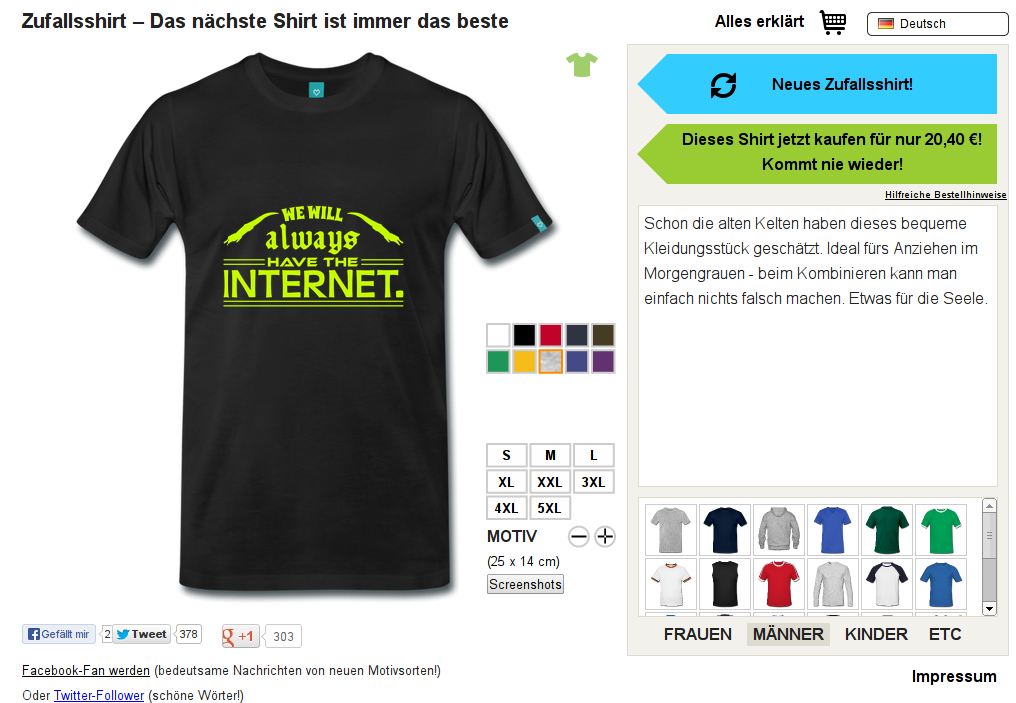
\includegraphics[height=0.8\textheight]{resources/zufallsshirt}
        \caption{Beispiel für kundenspezifische Anwendung: zufallsshirt.de}
    \end{figure}
\end{frame}
